\section{Project Review}
This project has faced some significant delays.
As discussed in my progress report, in the first half of this project, I had 
significant difficulty's with the implementation of the FFT.
This difficulty was resultant of my initial lack of knowledge about Agda,
a language I have not worked with previously, but was overcome after attempting
four different implementation techniques.

After the progress report, however, I faced more difficulties.
I initial believed that the proof equating the DFT and FFT would
be somewhat trivial, I was very much mistaken.
The final proof shown previously, and in the attached files was the result of a 
large number of iterations which changed both the preposition, and the chain of
reasoning.

One major issue I faced was that my initial preposition, as was shown in my 
progress report, did not perform reindexing over the input vector for the DFT, 
as was shown in \ref{sec:proof}.
I spent a large amount of time attempting to complete the proof without noticing
this issue, and only discovered this issue when I formed a contradiction.
This time was still helpful in the long run.
This is because it greatly helped my understanding of proofs in Agda, 
allowing me to experiment with a large number of proof tactics, some of which
I made use of in the final proof.
So much time was lost to this issue, and the burnout it caused, that
I was required to apply for an extension which allowed for the proof to be
completed, and report written.

As seen previously, my final proof forms a strong relation between the DFT
and FFT, providing a guarantee of the correctness of the FFT.
This was the main goal of my project brief.
However, because so much time was lost to a plethora of issues, I was unable to 
properly investigate \verb|c| code generation.
This was an additional, but non guaranteed, goal in my project brief which I 
had hoped would be achievable.

With this in mind, my original and my updated Gantt chart can be found in 
figure \ref{fig:gantt_halfway} and \ref{fig:gantt_final}.
\begin{landscape}
    \begin{figure}
        \centering
        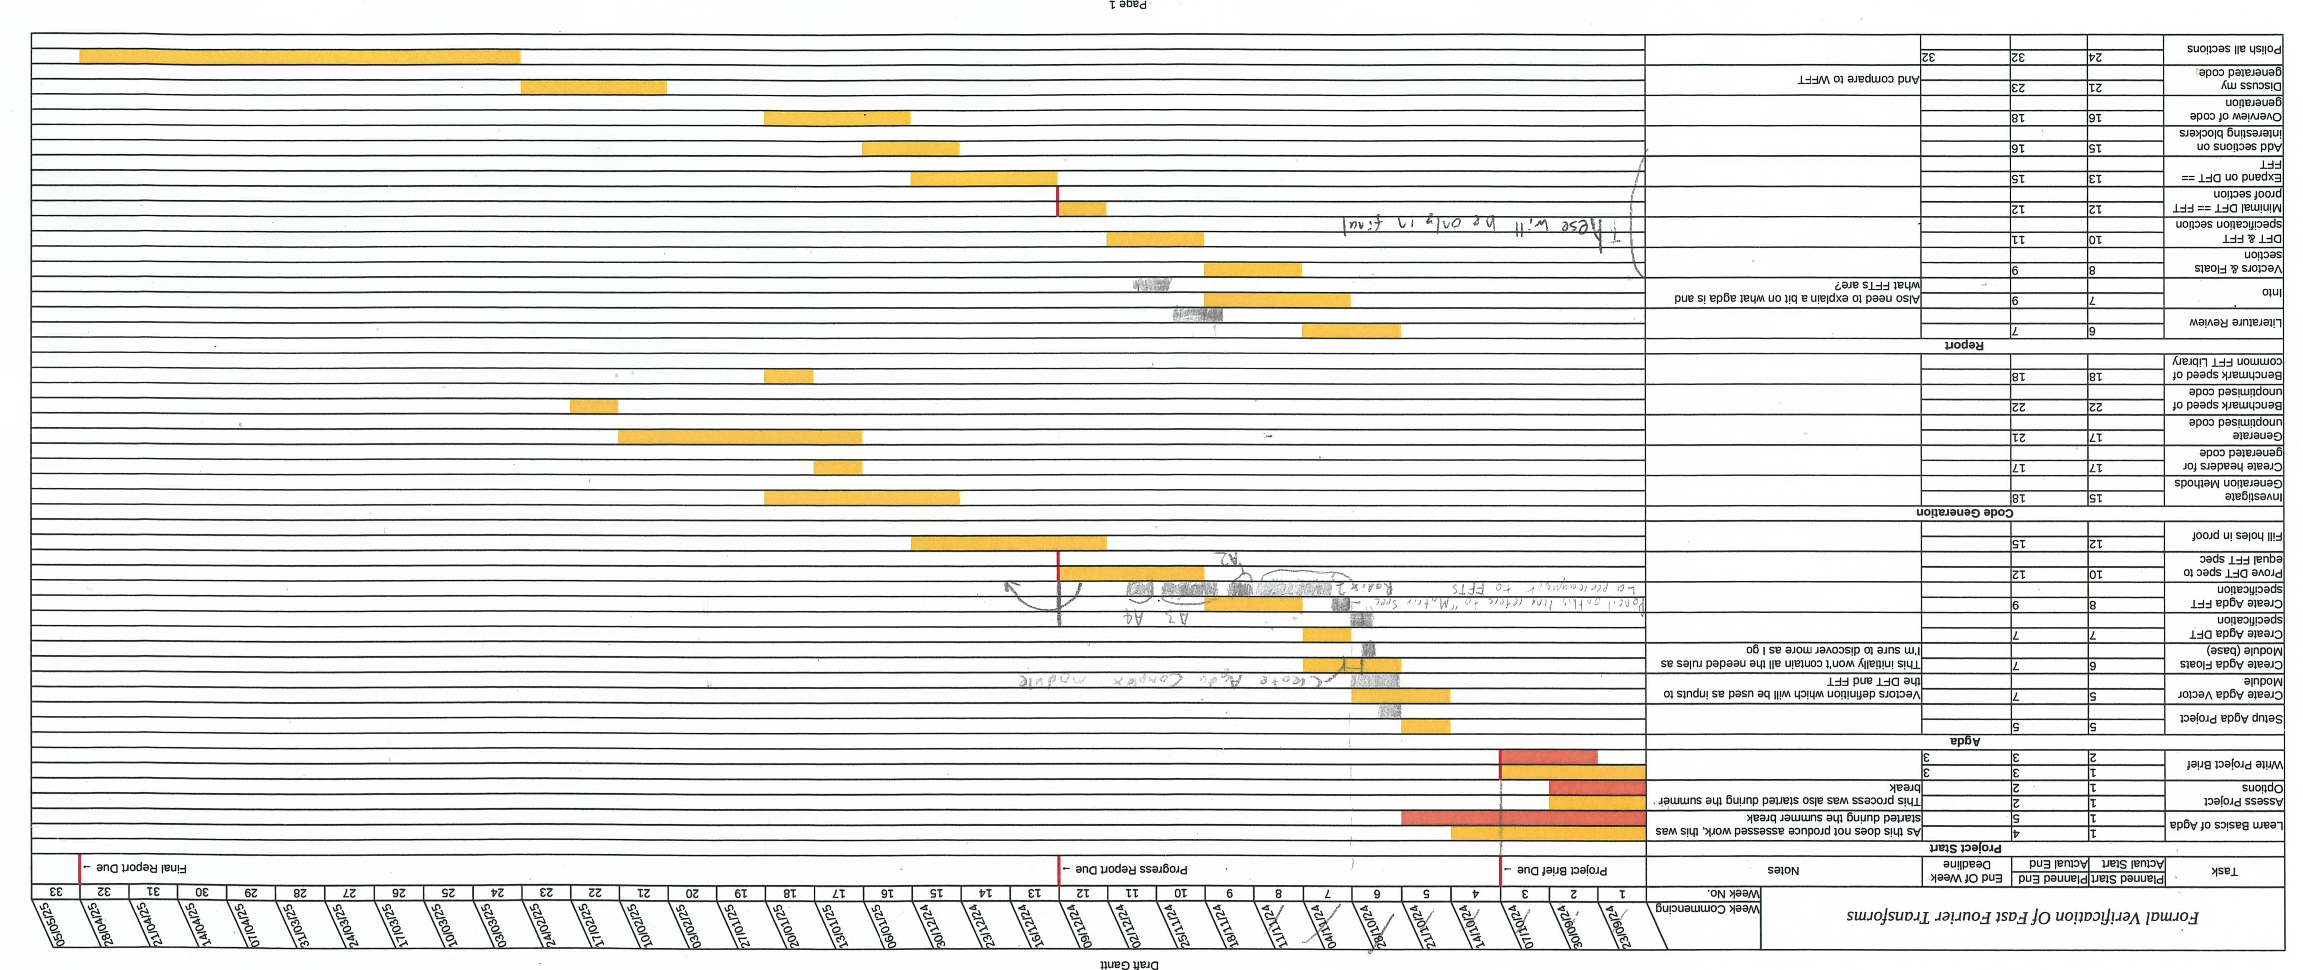
\includegraphics[angle=180, width=\linewidth]{Thesis/GanttHalfway.pdf}
        \caption{Gantt chart for the first half of the project}
        \label{fig:gantt_halfway}
    \end{figure}
\end{landscape}
\begin{landscape}
    \begin{figure}
        \centering
        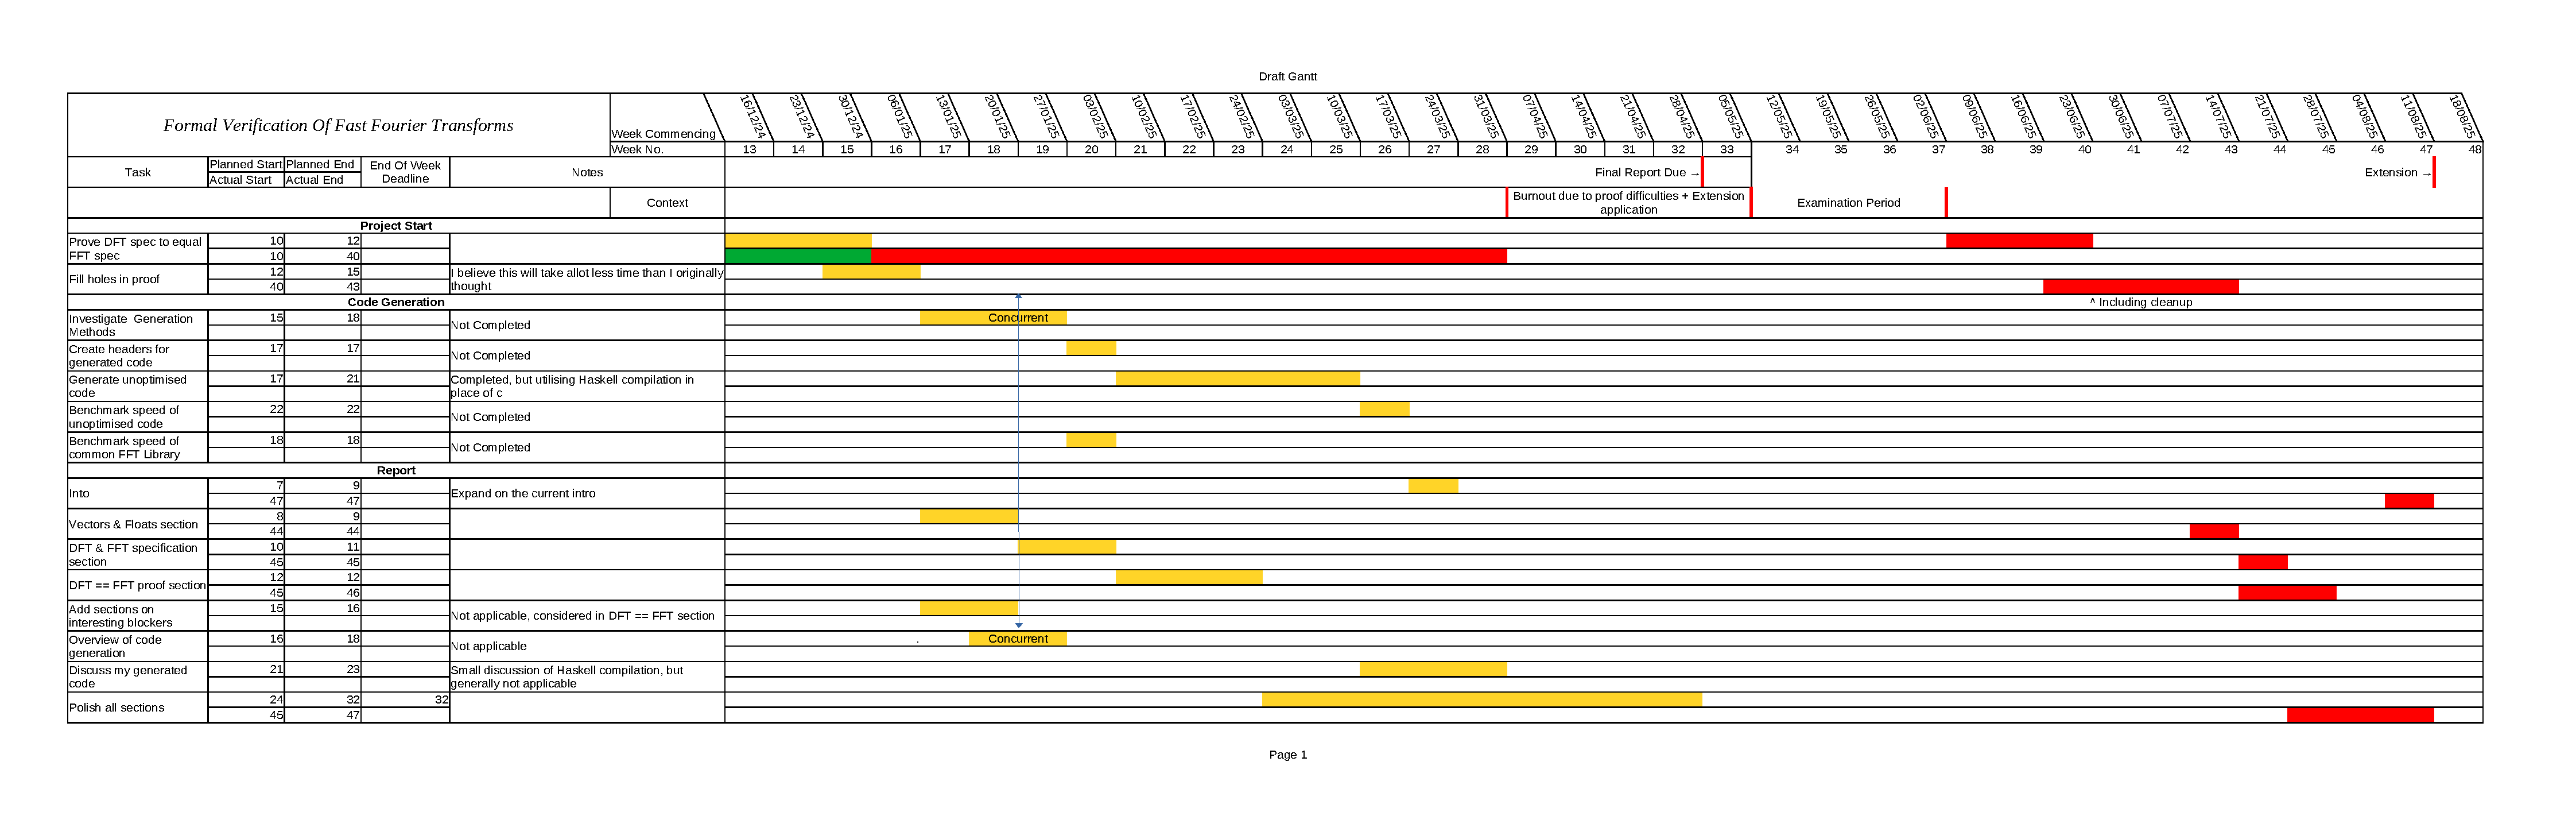
\includegraphics[width=\linewidth]{Thesis/GanttFinal.pdf}
        \caption{Final Gantt chart for the second half of the project}
        \label{fig:gantt_final}
    \end{figure}
\end{landscape}

